\documentclass[brazil]{abnt}
\usepackage[utf8]{inputenc}
\usepackage[brazil]{babel}
\usepackage{listings}

\usepackage{courier}
 \lstset{
         basicstyle=\footnotesize\ttfamily, 
         numberstyle=\tiny,          
         numbersep=5pt,              
         tabsize=2,                  
         extendedchars=true,         
         breaklines=true,            
         keywordstyle=\color{red},
                frame=b,         
         stringstyle=\color{white}\ttfamily, 
         showspaces=false,           
         showtabs=false,             
         xleftmargin=17pt,
         framexleftmargin=17pt,
         framexrightmargin=5pt,
         framexbottommargin=4pt,
         backgroundcolor=\color{lightgray},
         showstringspaces=false      
 }
 \lstloadlanguages{
         %[Visual]Basic
         %Pascal
         %C
         C++
         %XML
         %HTML
         %Java
 }

\usepackage{color}
\usepackage{xcolor}
\usepackage{caption}
\usepackage{graphicx}
\usepackage{wrapfig}
\DeclareCaptionFont{white}{\color{white}}
\DeclareCaptionFormat{listing}{\colorbox{gray}{\parbox{\textwidth}{#1#2#3}}}
\captionsetup[lstlisting]{format=listing,labelfont=white,textfont=white}

\makeatletter
\usepackage{babel}
\makeatother
\begin{document}

\autor{Renato dos Santos Cerqueira}
\titulo{Title Placeholder}
\orientador{Adriano Joaquim de Oliveira Cruz}
\comentario{Monografia apresentada para obtenção do Grau de Bacharel em Ciência da Computação pela Universidade 
Federal do Rio de Janeiro.}
\instituicao{Departamento de Ciência da Computação \par Instituto de Matemática \par Universidade Federal do Rio de Janeiro}
\local{Rio de Janeiro - RJ, Brasil}
\data{21/12/2012}

\capa
\folhaderosto

\begin{folhadeaprovacao}
Monografia de Projeto Final de Graduação sob o título \textit{``\ABNTtitulodata''},
defendida por \ABNTautordata~e aprovada em \ABNTdatadata, no Rio de Janeiro,
Estado do Rio de Janeiro, pela banca examinadora constituída pelos
professores: \setlength{\ABNTsignthickness}{0.4pt}

\assinatura{Prof. Ph.D. Adriano Joaquim de Oliveira Cruz\\ Orientador} \assinatura{???\\ Universidade ???} \assinatura{???\\ Universidade ???}
\end{folhadeaprovacao}

\begin{resumo}
O objetivo deste trabalho é fazer um \textit{engine} de jogo para o \textit{videogame Nintendo DS\texttrademark} e também um editor de fases 
e configurações, como seria feito numa equipe de desenvolvimento de um jogo grande, dando a possibilidade aos \textit{designers} 
de fazerem seus \textit{sprites} e criarem as fases com eles, sem que fosse necessário mexer com códigos.
\end{resumo}

\begin{abstract}
The objective of this paper is to make a game engine to the Nintendo DS\texttrademark system and a level and configurations editor, as it
would be done in a development team in a big game, giving designers the possibility to make their sprites and create their levels 
without touching actual source code.
\end{abstract}

\chapter*{Dedicatória}

\chapter*{Agradecimentos}

\tableofcontents{}
\listoffigures
\listoftables

\chapter{Introdução\label{cap:introducao}}

\vfill{}
\begin{flushright}{}``\emph{Não há fé inabalável senão aquela que}\\
\emph{pode encarar a razão face a face, em}\\
\emph{todas as épocas da Humanidade.}''\\
{\small Allan Kardec}\end{flushright}{\small \par}
\vfill{}

Neste capítulo são apresentados o objetivo desta monografia e a estrutura
da mesma.
\newpage


\section{Objetivo deste trabalho}

É comum ver retrospectivas lembrando da evolução dos jogos ao longo dos últimos anos. Jogos eletrônicos, como é sabido, são coisas relativamente recentes, sendo o primeiro exemplo conhecido de 1947, quando Thomas T. Goldsmith Jr. e Estle Ray Mann introduziram sua patente para um Dispositivo de Entretenimento usando Tubo de Raios Catódicos.

No entanto, muita coisa mudou nas poucas décadas da existências dos jogos eletrônicos. Quando vemos jogos produzidos na época do Atari 2600 e Magnavox Odyssey, estes eram criações de um único desenvolvedor, muitas vezes em períodos curtos de tempo, sem nem ao menos identificar o time de desenvolvimento. Era comum a aparição de \textit{Easter Eggs} que os desenvolvedores usavam para tentar identificar a sua criação.

Hoje em dia, porém, a indústria de jogos sendo a grande indústria que é, conta com superproduções com uma quantidade quase infindável de desenvolvedores, designers, criadores de fases, dentre outros tantos profissionais trabalhando cada um com sua especialidade.

Neste trabalho o que tentamos fazer é nos inserir um pouco no contexto desses times de criação modernos, vendo apenas uma pequena parte dessa tão grande cadeia de trabalho: a criação de ferramentas para facilitar a interação entre equipes de ramos diferentes. Mais especificamente, tentamos criar um jogo em duas dimensões, do tipo plataforma para o videogame portátil Nintendo DS. E tentamos fazer com que a engine que roda o jogo seja mais fácil de reutilizar através de ferramentas de criação de fases e de configuração do personagem, itens, dentre outras coisas que compõe o mundo do jogo.

Nosso objetivo, porém, é fazer o papel do desenvolvedor. E somente criar as ferramentas, imaginando como os outros times as usariam.

\section{Estrutura da monografia}

No capítulo~\ref{cap:engine} é apresentado o estado da arte
na área de segurança de redes ...


\chapter{A criação do jogo\label{cap:engine}}

\vfill{}
\begin{flushright}{}``\emph{Navegar é preciso, viver não.}''\\
{\small Luís de Camões}\end{flushright}{\small \par}
\vfill{}

Neste capítulo é apresentado o desenvolvimento da parte para o portátil Nintendo DS.
\newpage


\section{Introdução}

O que é exatamente um jogo de plataforma em duas dimensões? Podemos pensar em exemplos clássicos, como Super Mario World para o Super Nintendo, ou Sonic The Hedgehog para o Sega Mega Drive.

Nem todos os jogos plataforma são em duas dimensões. Mas vamos aqui nos focar num jogo plataforma em duas dimensões para facilitar o entendimento e o desenvolvimento de soluções. Nessa modalidade, uma característica comum presente em muitos jogos é o uso de \textit{tiles}, figuras de tamanho pré-definido, que compõem todo o mundo, como um grande quebra-cabeças. Nesse tipo de jogo, todos os objetos costumam ser feitos da combinações de sprites e muitas vezes um sprite é usado mais de uma vez em diferentes posições, para vários inimigos, por exemplo. Já os tiles são usados para compor o cenário, como pequenos tijolos.

Podemos definir um jogo de plataforma 2D por suas características comuns: o jogador controla um personagem que se movimenta para os lados, pode ou não saltar, ter ou não algum tipo de arma e em geral o objetivo é percorrer uma série de fases derrotando pequenos inimigos, para ao final derrotar algum grande inimigo e recuperar alguma coisa. Claro que essa é uma definição bem aberta, e é nela que vamos tentar nos inspirar ao escrever a parte que será executada no Nintendo DS.

Nosso objetivo é criar uma engine que leia algum tipo de arquivo de configuração, onde estarão detalhadas informações sobre quais são as imagens que compõem o personagem principal (ou personagens, no caso de haver uma escolha); informações sobre os inimigos como por exemplo a qual tipo de movimento ele obedece; descrição dos itens, como por exemplo qual efeito ele causa no personagem principal ou nos inimigos e informações sobre as fases, posicionamento de itens, inimigos e as imagens que as compõem.

\section{O processo criativo}

Na última seção, definimos o nosso objetivo. Assim, sabemos as características que queremos alcançar ao fazer nosso jogo. Devemos então começar a buscar ferramentas para alcançar o nosso objetivo. Começamos então nos focando nos elementos mais básicos: vamos pensar em como desenharemos o mundo, ignorando a existência dos inimigos e do jogador. Vamos pensar em como desenharemos o plano de fundo e os elementos imóveis do mundo.

Tentaremos seguir a idéia apresentada em \cite{mameri06culling}, cuja aplicação é direta para nós.

Enquanto não criamos o editor de fases, faremos uma pequena demonstração carregando uma matriz manualmente em nosso código, bem simples, delimitada por caracteres que representam determinados \textit{tiles}.

Estamos usando o kit de desenvolvimento \textit{homebrew}\footnotemark para o Nintendo DS, e com ele, a PALib, uma biblioteca que facilita o uso dos recursos de hardware do DS, que são um pouco limitados e curiosos, devido aos seus dois processadores e telas.

\footnotetext{O termo Homebrew se refere ao desenvolvimento com o uso de um kit de desenvolvimento extra-oficial, produzido por uma comunidade. Muitas vezes o kit de desenvolvimento oficial tem custo proibitivo e é voltado somente para grandes empresas de desenvolvimento. Desenvolvedores que queiram desenvolver em casa se valem desses kits não-oficiais, muitas vezes de código aberto, que são desenvolvidos em geral fazendo algum tipo de engenharia reversa no hardware original.}

Ao investigarmos a fundo, descobrimos que o DS suporta mapas com \textit{tiles}, ou seja, podemos criar um mapa e depois desconstruí-lo em pequenas imagens que serão repetidas várias vezes. Vamos então descobrir como podemos usar dessa característica. 

\subsection{Engine: O formato de background}

Investigamos o formato que é aceito pelo DS, em \cite{DSSpec}. Quando uma figura é colocada como plano de fundo, precisamos de quatro partes:

\begin{itemize}
 \item Arquivo Pal\\
 Neste arquivo, temos informações sobre a paleta usada no arquivo. São descritas todas as cores contidas no arquivo. O padrão é de 256 cores. O Formato usado no arquivo é A1B5G5R5, o que significa que tem um bit para o caso da cor ser transparente, 5 para o verde, 5 para o azul e 5 para o vermelho. A primeira cor no arquivo é a cor usada como transparência.
 \item Arquivo Tiles\\
 Neste arquivo, ficam os tiles, cada um de 8x8 pixels. Cada pixel do tile referencia uma cor do arquivo Pal. Neste arquivo, os tiles são escritos em blocos (vetores) de 64 bits. 
 \item Arquivo Map\\
 Neste arquivo, fica o mapa do background, ele referencia os tiles. Os bits 0-9 indicam o tile, o bit 10 indica se é espelhado na horizontal e o bit 11 indica se é espelhado na vertical.
 \item Arquivo .c\\
 Este arquivo constrói a struct que será usada no programa, informa algumas coisas como o tipo do mapa, o seu tamanho, os ponteiros para as regiões onde ficaram os três arquivos acima depois de linkados, tamanho do tiles em bytes e tamanho do map em bytes. 
\end{itemize}

Veja a listagem de código \ref{list:exemplobg}

Temos alguns detalhes a discutir nesse ponto. Como visto em \cite{DSSpec}, o DS tem mais de um formato de background, o que está descrito acima é o mais simples - e menos poderoso - dentre eles. Escolhemos ele como ponto de partida, para, se necessário, implementar os outros. Por exemplo, existem modos de usar mais de um arquivo de paleta, ou ainda usar mais tiles, mas sem o espelhamento. Ignoraremos esses outros formatos e modos, e nos focaremos no que está descrito acima.

Portanto, precisaremos que a nossa ferramenta dê a saída nesse formato. Por enquanto, para os testes, pensamos em usar ferramenta que vem junto com o kit de desenvolvimento, ela só converte uma imagem já pronta (ou seja, um mapa que já tenha sido desenhado) para este formato. Mas assim poderíamos fazer testes com relação a movimentação do background. No entanto, é muito difícil editar os arquivos de background manualmente, de modo que teremos de dar início a ferramenta de edição antes do esperado. Vamos começar fazendo ela como uma simples ferramenta de edição de background.

\section{GFXTool: A ferramenta de edição gráfica}
Começaremos então a criar a ferramenta. A idéia é que tenhamos uma área principal, onde será mostrado o que temos atualmente no mapa, uma área na lateral onde estarão os tiles que o usuário poderá usar para compor o background e algum botão que faça possível que o usuário edite, no próprio programa, os tiles. Ou crie novos.

Comecemos então por uma idéia básica, a de deixar o usuário importar uma imagem já pronta, e que o programa identifique os tiles contidos na imagem. Desta maneira, poderemos usar uma fase já pronta para fazer nossos testes, e o usuário poderia migrar um trabalho anterior para a nova engine. Numa grande empresa, poderia ser o caso de estar havendo uma adaptação de um jogo de uma plataforma antiga para o Nintendo DS.

\begin{figure}[h]
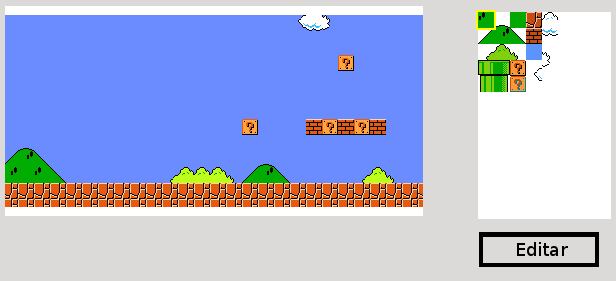
\includegraphics[width=\linewidth]{imgs/mockup.png}
\caption{Uma idéia da nossa interface} 
\end{figure}

Precisamos então decidir como faremos a interface. Como a parte do código da engine para o DS deverá ser feito em C++, pensamos que o ideal seria que o resto do projeto também fosse feito em C++, assim mantemos um certo padrão de linguagem. Com isso, buscamos as alternativas para a interface.

Como queremos que o projeto seja utilizável tanto em Windows, quanto em Linux, que será nossa principal plataforma de desenvolvimento, precisamos escolher uma biblioteca gráfica que suporte os dois sistemas operacionais e cujo custo de trocar de um pra outro seja muito baixo, ou seja, que não seja necessário reeescrever código para isso.

A solução que encontramos é utilizar a biblioteca Qt. A IDE para criação de interfaces, o QtCreator, deixa que as interfaces sejam criadas somente arrastando componentes e em seguida associando cliques a funções. E usando as funções do Qt para fazer as tarefas, o custo de troca entre Windows e Linux é basicamente zero. Falaremos mais sobre o porque da decisão da biblioteca no Anexo \ref{ferramentas-qt}.

Assim, fazemos a primeira janela do nosso programa, e o resultado é bem parecido com o que nós pensamos.

\begin{figure}[h!]
\centering
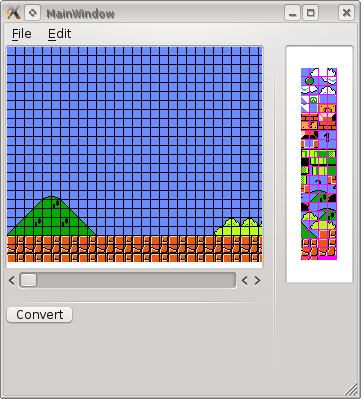
\includegraphics{imgs/mainwindow_1.png}
\caption{A nossa primeira interface} 
\end{figure}

Com a nossa interface definida, agora temos que nos preocupar em carregar o arquivo. Vamos considerar primeiro o problema de ler um arquivo já pronto e conversão desse arquivo para um formato do tipo ``mapa de tiles'', onde nós identificamos os tiles, e iremos compor o background a partir desses tiles. Fazemos isso com o código \ref{list:tilesv1}.

Vamos entender o que fazemos nesse código. A leitura da imagem fica por conta do Qt. Preenchemos o fundo do grid que vai conter nosso background com preto, em seguida, iteramos por toda a imagem, dividindo-a em quadrados de 8x8, ou seja, nossos tiles. Em cada um desses quadrados, identificamos se esse tile já foi incluído no nosso vetor de tiles. Se já, pegamos o índice desse vetor caso contrário, incluímos no vetor de tiles. Depois dizemos que nessa posição do background está o tile com esse índice. 

Inicialmente, não deixamos que o usuário amplie o mapa, ou seja, a imagem que ele carregar inicialmente tem que ser composta por tiles e já do tamanho final do mapa. Nossa intenção para depois, no entanto, é que o usuário possa criar um mapa vazio e carregar somente o conjunto de tiles. Do contrário, nosso software se resumiria a ter a mesma função da ferramenta já existente, a PAGfx, somente com uma interface mais rebuscada.

Como já comentamos, o hardware do DS suporta que pedaços de mapa sejam espelhados, tanto na vertical quanto na horizontal. No nosso código, não tratamos nenhum desses casos. Esse problema será visto mais adiante. No momento estamos mais preocupados em ter algo que permita que exportemos os backgrounds para que possamos começar a trabalhar na engine.

Agora que já lemos o background, temos que implementar as seguintes funções: seleção de tiles, usar o tile selecionado para pintar no mapa e exportar o mapa para o formato do DS. Como já exibimos na pequena janela o tile, basta que associemos os eventos de clique à janela, para que possamos implementar a funcionalidade de seleção de tiles.

Nós em primeiro lugar fizemos um código bem rudimentar, que simplesmente achava a posição do tile a partir da posição que o usuário havia clicado, e desenhava um quadrado ao redor dessa posição. No entanto, ele desenhava múltiplos quadrados, no caso do usuário sair clicando, e não funcionava no caso em que o usuário clicava duas vezes no mesmo quadrado.

Mexemos no código até que o usuário pudesse selecionar um tile com um clique, e desfazer a seleção clicando novamente. E também passamos a guardar a informação sobre o índice do tile selecionado. Afinal, isso seria necessário para quando quiséssemos pintar usando o tile selecionado. Uma funcionalidade interessante seria selecionar grupos de tiles, mas nós decidimos não a implementar num primeiro momento.

\chapter{Conclusões e trabalhos futuros\label{cap:conclusao}}

\vfill{}
\begin{flushright}{}``\emph{Nada se cria, nada se perde, tudo se
transforma.}''\\
{\small Lavousier}\end{flushright}{\small \par}
\vfill{}

Neste capítulo é apresentado as conclusões e alguns trabalhos futuros
...
\newpage


\section{Conclusões}

{\bf Alguns itens interessantes para a conclusão de um projeto de graduação}

Qual foi o resultado do seu trabalho? melhora na área, testes positivos ou negativos?
Você acha que o mecanismo gerado produziu resultados interessantes?
Quais os problemas que você encontrou na elaboração do projeto?
E na implementação do protótipo?
Que conclusão você tirou das ferramentas utilizadas? (heurísticas, prolog, ALE, banco de dados).
Em que outras áreas você julga que este trabalho seria interessante de ser aplicado?
Que tipo de continuidade você daria a este trabalho?
Que tipo de conhecimento foi necessário para este projeto de graduação?
Para que serviu este trabalho na sua formação?


\bibliographystyle{abnt-alf}
\bibliography{PF}


\anexo

\chapter{Listagens de código}

\lstinputlisting[caption=Exemplo de arquivo de mapa de background .c:,label=list:exemplobg]{codigos/exemplo_bg.c}

\lstinputlisting[caption=Lendo os tiles e os identificando (v1),label=list:tilesv1]{codigos/tiles.cpp}

\chapter{Ferramentas utilizadas}

\section{Qt}
\label{ferramentas-qt}




\chapter{Ferramentas utilizadas}

Foi feita uma análise de algumas ferramentas que são muito usadas
por atacantes (hackers) para a confecção de ataques. Estas ferramentas
são muito úteis em vários aspectos, tais como: (1) o levantamento
de informações sobre o alvo, (2) que tipo de serviços estão disponíveis
no alvo, (3) quais as possíveis vulnerabilidades do alvo, entre outras
informações. As ferramentas analisadas foram o \emph{nmap}~,
o \emph{nessus}~, o \emph{saint}~, além
de alguns comandos de sistemas operacionais (UNIX-Like e Windows-Like)
usados para rede, tais como o \emph{ping, nslookup e whois}. 
\end{document}
